\section{Modelling concept\label{sec:model_concept}}

\subsection{Model type}
\par{
    The central model concept is the use of a 2D \acrfull{cnn} to provide 3D segmentation masks, trained on point annotated data.
    Out-of-the-box pre-trained 2D networks are available, with weights pre-trained on public datasets\footnote{\label{footnote:Imagenet}For example, weights trained on the ImageNet dataset. 
    This dataset consists of over $14.10^6$ images of more than $2.10^4$ categories.}.
    An alternative approach would be to use 3D networks, which is a logical choice for volumetric data, with the apparent advantage that the 3D convolution layers naturally take into account the volumetric structure of the data.
    One could argue that using 2D networks deprives the network of crucial \textit{context} information in the direction perpendicular to the slice it is analysing (this work tries to meet this issue in section \ref{section:twoDplus} on page \pageref{section:twoDplus}).     
}

However, there are advantages to choosing 2D networks over 3D networks:
\begin{enumerate}
    \item Since the number of parameters (weights) to train scales exponentially with the kernel dimension, the number of parameters to train is considerably higher for a 3D \acrshort{cnn} compared to a corresponding 2D \acrshort{cnn}.
    \item The academic community has investigated 2D \acrlong{cnn}s for several years. The networks can be initialised with weights pre-trained on vast and diverse datasets (see remark \ref{footnote:Imagenet} on ImageNet). 
    These datasets indeed do not contain the specific classes nor the specific datatype investigated in this project. 
    However, the different convolution layers have proven to extract useful general features that allow the network to distinguish an extensive range of categories. 
    These features have proven to be sufficiently general to apply to new machine vision applications. This practice is called transfer learning.
    \item Although consecutive slices are strongly correlated, one has more data\footnote{There are more slices than volume segments in 1 image volume.} to train the networks. Certainly when considered in proportion to the number of weights to be trained.
\end{enumerate}

\subsection{Model training approach}

An approach used often in weakly supervised learning is the generation of \textit{ersatz} or \textit{pseudo} mask labels.
This project intends to use this approach too.

A scan volume can be sliced along 3 different axes: the transverse axis, the coronal axis and the sagittal axis (see figure \ref{fig:anatomicalPlains}). 
This means that 3 different models can be trained with the available point annotated data. 
Each of these 3 networks will have different context elements to segment the sliced images on.
The resulting segmentation volumes\footnote{The segmentation results of a stack of 2D slices can be combined to form a 3D segmentation volume.} of these three networks can then be combined to obtain a final segmentation volume.
This final segmentation mask, which should be as least as good as the best of the 3 individual model results, can then be used as pseudo masks to train a final \textit{fully supervised} network. 

\begin{SCfigure}[][htb]
    \centering
    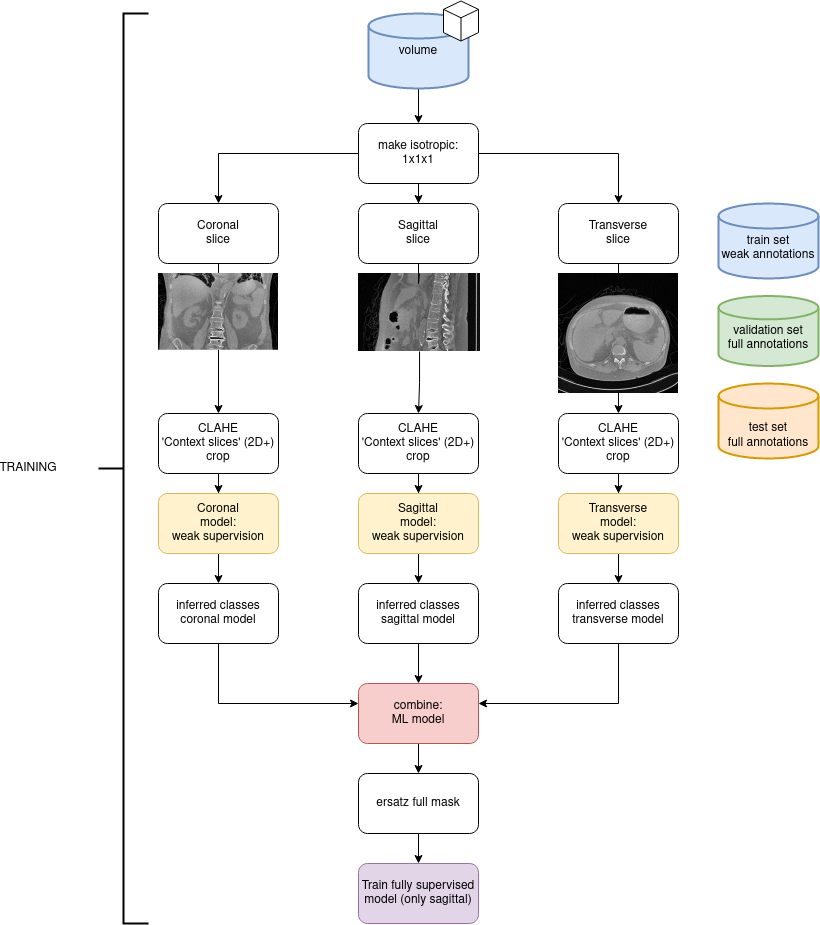
\includegraphics[width=.85\textwidth]{/home/thesis/images/Training_concept.png}
    \caption{\label{fig:model_training_concept}Illustration of the model training approach. 
    This is based on the conbination of 3 different models based on different volume slices.}
\end{SCfigure}

When the segmentation masks of a new, unknown volume need to be inferred, only this final model needs to be evaluated.
Only one set of slices along a single dimension needs to be generated and preprocessed to perform this evaluation.

\begin{SCfigure}[][htb]
    \centering
    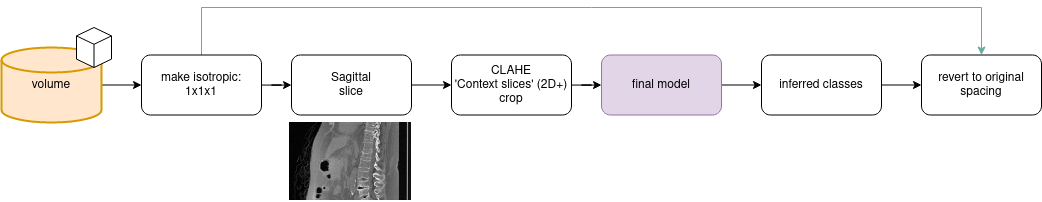
\includegraphics[width=.95\textwidth]{/home/thesis/images/Inference_concept.png}
    \caption{Inference step. Only one model needs to be evaluated in this step, the model that is trianed in the final step of the training procedure illustrated in figure \ref{fig:model_training_concept}.}
\end{SCfigure}